\documentclass[11pt,a4paper]{article}

\usepackage[ngerman]{babel}
\usepackage[ansinew]{inputenc}
\usepackage{amsmath}
\usepackage{gensymb}
\usepackage{breqn}
\usepackage{amsfonts}
\usepackage{amssymb}
\usepackage{url}
\usepackage[round, authoryear]{natbib}
%\usepackage{uml}
%\usepackage{graphicx}
\usepackage{appendix}

\usepackage[shellescape]{gmp}



% this is needed for forms and links within the text
%\usepackage{hyperref} 


% Title Page
\title{Agentenbasierte Modellierung am Beispiel des Ebro-Beckens in Spanien}
\author{Christopher Kittel}
\date{April - Juli 2013}

\begin{document}

\maketitle


\begin{abstract}
In dieser Arbeit wird ein agentenbasiertes Modell entwickelt, das im Bereich der Wasserversorgung die Schl"usselkomponenten (Angebot, Nachfrage, Infrastruktur, Umwelteinfl"usse) darzustellen, Verhalten auf Mikro\-ebene simulieren und auf Makroebene langfristige Tendenzen erkennbar machen kann.\\
Am Beispiel des Ebro-Beckens in Spanien stehen den AkteurInnen (Haushalte und Bew"asserungslandwirtschaften) verschiedene Handlungsoptionen zur Auswahl, die nachfrageorientierte umwelt"okonomische Politiken repr"asentieren. Ein einfaches Modell macht die Auswirkungen m"oglicher Umweltzust"ande und Akteursentscheidungen anhand von Kennzahlen wie Nutzen und Nutzenverlusten vergleichbar. \\
Ergebnisse lassen darauf schließen, dass nachfrageorientierte Policies dazu dienen k"onnen, die Resilienz sozio"okonomischer Systeme gegen"uber Angebotsschocks durch Umweltst"orungen zu erh"ohen. In diesem Modell ist dies vor allem durch adaptives Verhalten seitens der Haushalte und Landwirtschaften.
\end{abstract}


\newpage


\section{Einleitung}

Wasserversorgung ist ein komplexes System. Nach \citet{Moglia2010} liegen verschiedene Gr"unde daf"ur vor: Heterogenes Wassernutzungsverhalten, verschiedene Quellen und verschiedene Verwendungszwecke in Industrie, Landwirtschaft und privaten VerbraucherInnen, punktuelle Verschmutzungsquellen aufgrund der Landnutzung, Wasserstr"ome und Leckagen in einem komplizierten technischen System, zuf"allige Wettereinfl"usse und hydrologische Dynamiken. Die Komplexit"at der Wasserversorgung versch"arft die Problematiken, die auf physische und sozio"okonomische Systeme zukommen. Die UN hebt in ihrem Weltwasserbericht \citep{UN2012} die Notwendigkeit hervor, die Problematik "uber sektorale und nationale Grenzen der Wasserversorgung hinaus zu denken. Wasser ist Grundlage f"ur Energieerzeugung, Nahrungsmittelproduktion, Grundbed"urfnis der Menschen, und in "Okosystemen unersetzbar. Grenzu"bergreifende Flusssysteme sind immer wieder Ausl"oser f"ur diplomatische Verstimmungen\footnote{http://www.dw.de/wasserkrieg-zwischen-"Agypten-und-"Athiopien/a-16879225}. \\
Trotz ausf"uhrlicher Besch"aftigung verschiedener Fachgebiete gibt es auch aus "okonomischer Sicht noch offene Fragen. \cite{Castellano2008} nennen beispielsweise die Opportunit"atskosten die anfallen, wenn Wasser zum Erhalt von "Okosystemen genutzt werden soll, als bisher vernachl"assigten Aspekt an. \\
Bisherige Wege mit diesen Problematiken umzugehen basieren auf statistischen Methoden wie Regressionsanalysen, Zeitreihenanalysen und geo"-phy"-sikal"-ischen Modellen. Agentenbasierte Modelle k"onnen hier erg"anzend eingesetzt werden, um Kausalit"aten abzuleiten und so zu einem tieferen Verst"andnis der Systeme beizutragen \citep{Galan2011}. Agentenbasierte Modelle vereinigen die F"ahigkeiten anderer Modellierungstechniken, und sind in der Lage dynamische Feedbacks, evolution"are Prozesse, autonomes Verhalten, heterogene und interagierende Akteure sowie adaptives Entscheidungsverhalten zu simulieren \citep{Heckbert2010}.\\
Mit dem Themenfeld der Wassermodellierung haben sich, unter Verwendung dieser und "ahnlicher Methoden, verschiedene Studien auseinandergesetzt: \cite{Angus2009} haben die Auswirkungen des Klimawandels auf Bangladesch simuliert, \cite{Galan2011} untersuchten die Auswirkungen von Migration und Urbanisierungsprozessen auf Wassernutzung, \cite{Wise2012} erstellten ein Modell zur Untersuchung kleinstrukturierter Landwirtschaft. \\

Das in dieser Arbeit entwickelte Modell ist auf den Fall ausgerichtet, dass angebotsorientierte Maßnahmen nicht mehr ausreichen und ein Zustand relativer Knappheit eintritt. Es soll in erster Linie simulieren, wie verschiedene Akteure auf derartige Knappheiten reagieren. Die theoretische Problembeschreibung erfolgt in Kapitel \ref{sec:Konzeptionierung}. Dazu ist es notwendig, über die Betrachtung einzelner Teilbereiche hinauszugehen, und drei verschiedene Subsysteme (Umwelt, Landwirtschaft, urbane VerbraucherInnen) zu integrieren. Die Entwicklung des Modells und Integration der Fragestellung erfolgt in Kapitel \ref{sec:Umsetzung}.\\
Das Modell simuliert verschiedene Umweltzust"ande und ihre Auswirkungen auf die Wasserverf"ugbarkeit. Maßnahmen k"onnen dahingehend evaluiert werden, wie gut sie nat"urliche Versorgungsschwankungen ausgleichen, und so die Versorgungsunsicherheiten seitens st"adtischer und landwirtschaftlicher Verbraucher minimieren. Die Analyse und Diskussion des Modell-Outputs erfolgt in Kapitel \ref{sec:Modelloutput}.


\section{Konzeptionierung der Fragestellung}
\label{sec:Konzeptionierung}

\subsection{Definitionen}

Knappheit im weiteren Sinne wird in diesem Modell als Zustand definiert der dann auftritt, wenn die Gesamtnachfrage das Gesamtangebot "ubersteigt. Im engeren Sinne kann Knappheit definiert werden, wenn die individuell verf"ugbare Menge einen bestimmten Grenzwert unterschreitet. Dies kann aus zwei unterschiedlichen Gr"unden auftreten: Zum einen physikalische Knappheit, wenn die vorhandene Menge Wasser in einem bestimmten Gebiet nicht ausreicht, um die Bed"urfnisse der lokalen Bev"olkerung zu decken; zum anderen "okonomische Knappheit, erzeugt durch institutionelle oder finanzielle Beschr"ankungen \citep{UN2012}.\\
Die UN hat Grenzwerte f"ur definiert, ab welchen in einem Gebiet Wasserstress bzw. Wasserknappheit im engeren Sinne vorherrschen. Sie betrachtet dazu das Verh"altnis Wasser - Bev"olkerung. Wenn die pro-Kopf-Versorgung unter 1.700 $m^3$ pro Jahr sinkt, liegt Wasserstress vor. Unter 1.000 $m^3$  liegt Wasser\-knappheit vor, und unter 500 $m^3$ pro Jahr liegt absolute Knappheit vor.\\

In dieser Arbeit wird f"ur Wasserstress eine alternative Metrik verwendet: Wasserstress wird hier als das Verh"altnis von verbrauchter zu erneuerbar vorhandener Menge Wasser definiert. Es ist damit ein Wert zwischen 0 und gr"oßer 1, wobei Werte gr"oßer 1 nur auftreten k"onnen, wenn auf vorhandene Reserven zugegriffen werden kann.

Resilienz ist ein Konzept, dass in diesem Modell nur am Rande verwendet wird, jedoch Motivation f"ur viele Bem"uhungen der Modellierung und Analyse ist. In diesem Modell wird die "okologische Definition von \cite{Hawes2006} verwendet: ''Ecological Resilience is the amount of disturbance required to change from one
steady or cyclic state to another.'' Im Fokus steht dabei der Funktionserhalt, und Analysen konzentrieren sich st"arker auf Faktoren die Instabilit"aten und St"orungen verursachen. Systeme k"onnen in dieser Definition mehrere stabile Zust"ande besitzen.


\subsection{Problemstellung aus "okonomischer Sicht}

Die Wasserversorgung steht zuk"unftig vor großen Herausforderungen. Zunehmende Umweltvolatilit"at durch Klimawandel, zunehmende Urbanisierung, Wasserverschmutzung durch Industrie und intensive Landwirtschaft, sinkende Gew"asser- und Grundwasserspiegel durch Bew"as\-serungs\-land\-wirt\-schaft sind Faktoren, die Wasserressourcen belasten. Maßnahmen zur Sicherstellung ausreichender Versorgung waren bisher vor allem technischer Natur und angebotsorientiert. Diese beinhalten den beispielsweise den Bau von D"ammen, Kan"alen und Regulierungseingriffe in nat"urliche Gew"asser \citep{Olmstead2010}.\\

Die Aufmerksamkeit der "OkonomInnen hat sich in den letzten Jahren vor allem an die Nachfrageseite gewandt. \cite{Ruijs2008} untersuchten die Auswirkungen von unterschiedlichen Wasserpreismechanismen auf die Nachfrage in Brasilien. \cite{Wheeler2008} untersuchten Preiselastizit"aten in Australien. Die Auswirkungen verschiedener Preisstrukturen wurden ebenfalls von \citep{Olmstead2007} untersucht. Verschiedene Mechanismen, wie mit Wasserressourcen umgegangen werden kann, sind ebenso Forschungsobjekt geworden: \cite{Chong2006b} untersuchten ausf"uhrlich die Vor- und Nachteile von handelbaren Wasserrechten, und \cite{Nguyen2013} simulierten ein agentenbasiertes Modell des Wasserhandels unter asymmetrischen Informationen und Unsicherheit. Die "okonomischen Kosten des Fehlens von Wasserm"arkten wurde von \cite{Brennan2008} untersucht. \cite{Goetz2008} untersuchten die Alternative der Wasserallokation durch soziale ausgehandelte Regeln (Social Choice).\\

Wasserressourcen weisen einige charakteristische Probleme auf: Wasserpreise werden selten "uber M"arkte bestimmt, und geben Knappheiten nicht wieder. Dies l"asst sich darauf zur"uckf"uhren, dass urbane Wasserversorgung oft durch "offentliche Unternehmen gew"ahrleistet wird, die eine Monopolstellung besitzen und in ihrer Preisgestaltung auch politischer und sozialer Einflussnahme unterliegen.\\
Die Einf"uhrung eines Marktes wiederum erfordert eine Privatisierung von Wasserressourcen, was in vielen F"allen nicht erw"unscht ist. Dazugeh"orige Allokationsmechanismen sind meist eine politisch heikle Angelegenheit, und Eigentumsrechte sind ebenfalls kompliziert zu handhaben, da sie nicht immer klar verteilt oder eingrenzbar sind. Die Problematik wird versch"arft, wenn die Ressource ein Open-Access-Gut ist, welche rival und ohne Zugangsbeschr"ankungen vorliegt. Dies f"uhrt zur bekannten ''tragedy of the commons'' \citep{Hardin1968}.\\

F"ur die Modellentwicklung relevant, habt Olmstead bei der Gestaltung einer Nachfragefunktion des Haushaltssektors hervor, dass Grenzpreise, Einkommen und Variablen f"ur Haus\-halts\-pr"a\-ferenzen vorkommen m"ussen. Ebenso sollten sie Faktoren wie Saison oder Wetter enthalten. Eine von Olmstead durchgef"uhrte Literaturreview ergibt, dass die Haushaltsnachfrage mit Werten zwischen -0.38 und -0.64 preis\-in\-elastisch ist.\\
Da industrielle und landwirtschaftliche Verbraucher Wasser oft aus nicht gemessenen Quellen beziehen, ist hier die Datenlage schwierig. Um Wasser hier einen Wert beimessen zu k"onnen, muss das Grenzprodukt isoliert werden, wie es beispielsweise \cite{Salvador2011} f"ur das Ebro-Becken sch"atzten. Olmstead findet in ihrer Literaturreview auch bei Industrie und Landwirtschaft tendenziell Preisinelastizit"at vor, mit Werten zwischen -0.15 bis -0.98. Diese Werte schwanken je nach industriellem Sektor.\\

\subsection{Spezifika des Ebro-Beckens}
Im Ebrobecken unterliegt die Wasserversorgung besonders schwierigen Bedingungen. Hohe Evapotranspiration erschwert die Landwirtschaft, niedrige Niederschlage vor allem im Sommer erh"ohen die Abh"angigkeit von Reservoirs und erzwingen die Heranf"uhrung von Trink- und Brauchwasser aus den Randgebirgen. Das Ebro-Becken besitzt ein arides Klima und geh"ort zu den trockensten Regionen Europas, dennoch wird ein hohem Ausmaß Bew"asserungslandwirtschaft betrieben. Sowohl die Bev"olkerung als auch die Industrie und Landwirtschaft sind vom Wasser des Ebro-Flusssystems ab\-h"an\-gig. Durch die hohe Evapotranspiration spielen Niederschl"age kaum eine Rolle \citep{Salvador2011}, das Flusssystem speist sich vor allem aus den n"ordlich gelegenen Pyren"aen und dem s"udlich gelegenen iberischen Gebirge. Da die Evapotranspiration im Jahresgang mit 800mm die Niederschl"age von 300mm \citep{Penagos2007} "uberschreiten, f"uhrt dies tendenziell zu einer Austrocknung des Bodens und ohne Bew"asserung zum Verlust von Ackerland. Zur Sicherstellung der Wasserversorgung wurde in den letzten Jahrzehnten ein umfangreiches Netz aus Kan"alen und Wasserspeichern angelegt. Insgesamt gibt es im Ebro-Becken Wasserreservoirs mit einer Gesamtkapazit"at von 6.837 Hm$^{3}$. Das im Ebro-Becken bew"asserte Land stellt ein F"unftel der bew"asserten Fl"ache in Spanien dar und umfasst insgesamt 784.000 Hektar \cite{Salvador2011}.\\

Da die nat"urlichen M"oglichkeiten, Speicherbecken anzulegen allm"ahlich ersch"opft sind, und die zunehmende Wasserentnahme und Regulierung des Flusses zu negativen "okologischen Auswirkungen f"uhren \citep{Alcacer2005}, ger"at zunehmend die Nachfrageseite ins Blickfeld. Aus um\-welt\-"oko\-nom\-ischer Sicht stellen sich Fragen hinsichtlich der Auswirkungen von drohenden Wasserknappheiten, sowie m"oglicher Steuerungsmaßnahmen und ihr\-en Folgen. Diese Arbeit will einen Ansatz zur Untersuchung dieser Fragen erarbeiten, und in diesem Zuge das Potenzial agentenbasierter Modellierung zur Beantwortung dieser Fragen ausloten.

\subsection{Herangehensweise}
Die Problemstellung, die in dieser Arbeit behandelt wird, ist die Integration der vielschichtigen Problematiken der Wasserversorgung. Dabei wird ein Fokus auf nachfrageseitiges Verhalten und Regulierungsmaßnahmen gelegt. Dazu muss eine Definition von Knappheit in ein mathematisches Modell umgesetzt werden, einzelne Akteure wie Haushalte und Landwirtschaften m"ussen modelliert werden, und das Modell muss als Output "okomische Kennzahlen besitzen.\\
Das in dieser Arbeit konzeptionierte Modell wird vor die Herausforderung gestellt, Nachfrageverhalten zu simulieren. Basierend darauf k"onnen Kennzahlen wie aggregierter Nutzen, und durch Knappheit entgangener Nutzen erhoben werden. Angebots- oder Nachfrageseitige Regulierungen oder Anreize k"onnen im Hinblick auf ihr langfristiges Potenzial, Knappheiten zu verringern, untersucht werden, um so die geeignetsten Maßnahmen zu finden. Einflussfaktoren sind dabei das Nachfrageverhalten von privaten und landwirtschaftlichen Verbrauchern, sowie das Angebotsverhalten von "offentlichen und/oder privaten Anbietern. Das System bewegt sich dabei in einer stoch\-astisch modellierten Umwelt, um unkontrollierbare Schwankungen durch globale Klima- und lokale Wetterph"anomene einbeziehen zu k"onnen. Das Modell wird anhand der spanischen Ebro-Region modelliert und mit empirischen Daten initialisiert. \\

In seiner Grundfunktion beschreibt das Modell das Verbrauchsverhalten von Haushalten, sowie das Verbrauchsverhalten von Bew"asserungslandwirtschaften. Das Modell simuliert das grundlegende Verhalten des Systems, und erlaubt in erweiterter Funktion strategisches Verhalten, Lernprozesse und Marktmechanismen. Zur Entwicklung der Fragestellung wurde im weiteren auch das Szenario-Framework von \cite{Leenhardt2012} herangezogen.\\
Der Output sind Kennziffern die einen Vergleich physikalischer Werte wie pro-Kopf-Verbrauch und Verbrauch pro Hektar, sowie aus "okonomischer Sicht der Nutzen von Haushalten und Landwirtschaften erm"oglichen. Der Nutzen wird in diesem Modell jeweils abstrahiert von Wasserverbrauch bzw. Wasserproduktivit"at abgeleitet. Haushalte als auch Landwirtschaften erhalten dazu zwei Nutzenfunktionen. Exemplarisch f"ur nachfrageseitige Policies wird in diesem Modell adaptives Verhalten "uber zwei Lernfunktionen, die der Nutzenmaximierung dienen, simuliert.\\

Haushalte besitzen adaptives Verhalten in zwei Dimensionen: Variation der Haushaltsgr"oße, also der Anzahl der BewohnerInnen eines Haushalts, und Variation der technischen Effizienz, also die Verwendung wassersparender Haushaltsger"ate. Die Entscheidung, ob und in welcher Art diese Variablen ver"andert werden, wird anhand ihrer Auswirkung auf den Nutzen eines Haushalts berechnet. Haushalte versuchen ihren Nutzen zu maximieren und Kosten zu minimieren, indem ähnliche Agenten beobachtet werden. Das Verhalten erfolgreicherer Vertreter wird kopiert, und so verbreiten sich erfolgreiche Verhaltensweisen. \cite{Arbues2010} weisen darauf hin, dass die durchschnittliche Haushaltsgr"oße von Saragossa von 3,0 BewohnerInnen (1991) auf 2,2 BewohnerInnen 2008 gesunken ist. Eine gegenl"aufige Tendenz k"onnte zu niedrigerem pro-Kopf- und Gesamtverbr"auchen beitragen. \\
In diesem Modell k"onnen Landwirtschaften ihr Verhalten ebenfalls in zwei Dimensionen variieren, um ihren Nutzen zu maximieren und ihre Kosten zu minimieren. Zum einen hat die Auswahl der angebauten Nutz\-pflanze Auswirkungen auf Wasserverbrauch (Kosten) und Grenzproduktivit"at einer Einheit Wasser (Nutzen), zum anderen hat die Auswahl des technischen Bew"asserungssystems Auswirkungen auf den Wasserverbrauch. \cite{Varela-Ortega1998} kommen in ihrer Untersuchung dreier spanischer Regionen zum Ergebnis, dass hohe Wasserpreise zu Variationen in der Verteilung der Nutzpflanzen f"uhren k"onnen. Sie kommen ebenfalls zum Ergebnis, dass technologische "Anderungen nur geringen Einfluss auf Wasserverbrauch bei einer bestimmten Fruchtwahl haben, da f"ur jede Frucht nur bestimmte Kombinationen von Bew"asserungstechnik und -menge zum optimalen Ergebnis f"uhren.\\

Die jeweiligen Nutzenfunktionen werden im Abschnitt \ref{sec:Umsetzung} genauer erl"autert. Diese Arbeit st"utzt sich, was empirische Daten und "okonometrische Analysen betrifft, stark auf die Arbeiten von \cite{Arbues2010} und \cite{Salvador2011}, die sich mit den urbanen und agrarischen Verbrauchern im Ebro-Becken intensiv auseinandergesetzt haben. Der inhaltliche Aufbau der Arbeit wurde stark durch das Konzept-Framework von \cite{Grimm2010} beeinflusst, die ein ausgereiftes Werkzeug erarbeitet haben, das bei der Entwicklung eines agentenbasierten Modells sehr hilfreich ist.


\section{Umsetzung des Modells}
\label{sec:Umsetzung}
In diesem Abschnitt werden die einzelnen Funktionen des Modells erl"autert. Abschnitte \ref{sec:Akteure}, \ref{sec:Variablen}, \ref{sec:Skalierungen} und \ref{sec:Initialisierung} beschreiben die individuellen Agenten (Haushalte und Landwirtschaften), ihre Variablen und Parameter. \\
Drei Teilmodelle sind besonders relevant: Jeweils das individuelle Ent\-schei\-dungs- und Lern\-verhalten von land\-wirt\-schaft\-lichen Be\-w"as\-ser\-ungs\-ein\-hei\-ten und Haus\-halten "uber die konsumierte Wassermenge, und die Angebotsfunktion. Dar"uber hinaus gibt es noch ein Teilmodell f"ur die Simulation der Umwelt, das großteils stochastisch abl"auft. Die Beschreibung des Modells erfolgt hier in der logischen Abfolge, wie sie im Modell zu jedem der 1.040 Zeitschritte durchgef"uhrt wird.\\

\begin{enumerate}
\item Umweltfunktion
\item Angebotsfunktion
\item Nachfragefunktionen der Haushalte und Landwirtschaften
\item Knappheitsfunktion
\item Nutzenfunktionen der Haushalte und Landwirtschaften
\item Lernfunktionen der Haushalte und Landwirtschaften
\end{enumerate}

Zum Verst"andnis der Modellbeschreibung ist anzumerken, dass Funktionen auf zwei verschiedene Arten beschrieben werden. Zum einen in mathematischer Form, wenn sie aus aus anderen Studien zitiert und empirisch abgeleitet wurden. Zum anderen in verbaler Form, wenn sie als Hilfsfunktionen innerhalb des Modells modellinterne Zwischenergebnisse berechnen.

\subsection{Akteure, Variablen, Skalierungen}\label{sec:Akteure}
\subsubsection{Akteure}
Die atomarste Einheit des Modells wird Agent genannt, und repr"asentiert eindeutige oder abgetrennte Objekte (wenn passiv) oder Akteure (wenn aktiv). Ein Agent verh"alt sich individuell und kann mit anderen Agenten interagieren oder durch Umweltfaktoren beeinflusst werden. Agenten sind durch Variablen definiert, die sie von anderen Agenten unterscheiden und mitverfolgen lassen, wie sich der Agent "uber die Zeit ver"andert.\\

In diesem Modell werden zwei Klassen von handelnden Agenten eingesetzt: private Verbraucher (Haushalte) und landwirtschaftliche Verbraucher (Bew"asserungslandwirtschaften). Die nat"urliche und r"aumliche Umwelt wird, stark vereinfacht, durch Objekte im Modell repr"asentiert: Fl"usse und ihre Einzugsgebiete, sowie Umweltbedingungen wie Temperatur. Dar"uber hinaus werden bisherige technische Verbesserungen des Wasserangebots (Kan"ale und Staubecken) als Reservoirs aggregiert repr"asentiert.\\
Um im Modell eine gewisse realit"atsn"ahe bei gleichzeitiger Einfachheit zu erreichen, werden lediglich die zw"olf gr"oßten St"adte der Region einbezogen.  Diese hatten im Jahr 2006 1.531.647 EinwohnerInnen\footnote{http://www.ine.es/}. EinwohnerInnen werden im Modell auf 1.000 Agenten (Haushalte) verteilt, denen im weiteren Verlauf verschiedene Attribute, wie z.B. Einkommen, zugeordnet werden. Ein Haushalt im Modell steht also je nach Stadtgr"oße f"ur ca. 500 bis 1.500 EinwohnerInnen. Aus Gr"unden der Vergleichbarkeit erhalten alle Haushalte die gleichen Nachfrage- und Nutzenfunktionen.\\

Im Ebrobecken wird insgesamt eine Fl"ache von 784.000 ha Land be\-w"as\-sert, ein F"unftel der Gesamtackerfl"ache in Spanien \citep{Salvador2011}. Oberfl"achenbew"asserung ist mit 69 Prozent der Fl"ache die h"aufigste Technik, danach folgen Berieselung und Tropfbew"asserung mit 19 bzw. 12 Prozent. Insgesamt existieren im Ebro-Becken 1.746 Bew"asserungslandwirtschaften mit Fl"achen zwischen 1 und 50 ha, die Durchschnittsgr"oße liegt bei 10 ha. Auch hier wird die Anzahl der Landwirtschaften reduziert, sodass im Modell nur die 373 gr"oßten Landwirtschaften vorkommen, die zusammen 691.085 ha ausmachen (88 Prozent der Gesamtfl"ache).

\subsubsection{Variablen}\label{sec:Variablen}
Es gibt zwei Arten von Variablen, die notwendig ist um den Systemzustand zu jedem beliebigen Zeitpunkt abbilden zu k"onnen. Bestandsgr"oßen sind zeitabh"angig und werden durch Zu- oder Abfl"usse ver"andert. Stromgr"oßen sind zeitunabh"angig und repr"asentieren Ver"anderungen von Bestandsgr"oßen. Diese Variablen sollten so elementar definiert sein, dass sie nicht von andere Variablen abgeleitet werden k"onnen. Alle anderen Faktoren und Werte fließen als Parameter in das Modell ein. In diesem Modell ist die verf"ugbare Wassermenge eine globale Stromgr"oße. \\

\paragraph{Haushalte}haben als Bestandsgr"oßen die Haushaltsgr"oße (Anzahl der BewohnerInnen pro Haushalt), w"ahrend Nachfrage (Wasserkonsum in $m³$) und Nutzen Stromgr"oßen sind. Die Haushaltszusammensetzung als Bestandsgr"oßen wurden gew"ahlt um den Datenerfordernissen der Nachfragefunktion zu gen"ugen. Die Nachfrage als Wasserkonsum in Kubikmetern wurde als Stromgr"oße gew"ahlt, um das reale Verhalten abzubilden. Der Nutzen ist eine virtuelle Gr"oße die als Grundlage f"ur adaptives Verhalten dient, und um "okonomische Vergleiche zwischen Haushalten zu erm"oglichen.\\

In Tabelle \ref{tab:hh-description} werden die Eigenschaften der Haushalte zusammengefasst, wie sie zur Modellierung der Konsum- und Lernverhaltens ben"otigt werden. Die einzelnen Funktionen werden jeweils gesondert erl"autert.

\newline
\begin{tabular}{|l|l|l|r|}
\hline \textbf{Haushalte} & & & \\ 
\hline \textbf{Variablen} & \textbf{Typ} & Variablen & Beispielwerte \\ 
\hline pro-Kopf-Nachfrage & numerisch & $q_{it}$ & 90 - 150 l / Tag \\ 
\hline Kosten & numerisch &  $de_{it-2,4}$  & 80 - 200 EUR / Quartal \\ 
\hline Haushaltsgr"oße 1-5 & boolean & D1 - D4 & jeweils 0/1 \\ 
\hline Verm"ogen & numerisch & W & 5.000 - 126.000 EUR \\ 
\hline Warmwasserversorgung & boolean & CHW & 0/1\\ 
\hline Population & numerisch & pop & 500 - 1.500\\ 
\hline Altersstruktur & boolean & AG20, AG60 & jeweils 0/1\\ 
\hline Technologiefaktor & numerisch & TF & 1 / 1,1\\
\hline Nutzen & numerisch & $U_{h}$& 0 - 80\\
\hline Knappheits-Nutzen & numerisch & $U_{sh}$ & 0 - 40\\
\hline \textbf{Funktionen} & & & \\
\hline Nachfragefunktion & & Funktion (\ref{eq:household-demand}) & \\
\hline Nutzenfunktion & & Funktion (\ref{eq:household-utility-function}) & \\
\hline Lernfunktion & & Funktion (\ref{eq:household-learning-function}) & \\
\hline 
\label{tab:hh-description}
\end{tabular} 
\newline

\paragraph{Landwirtschaften}haben als Bestandsgr"oßen Grenzproduktivit"at pro Kubikmeter Wasser. Nachfrage und Nutzen sind Stromgr"oßen. Die Grenzproduktivit"at eines Kubikmeters Wasser (gemessen in Euro pro Kubikmeter) wurde durch \cite{Salvador2011} von der erreichten Ertragssteigerung bei verschiedenen Feldfr"uchten hergeleitet. Sie wurde gew"ahlt um die unterschiedlichen Landwirtschaften und technologischen Bew"asserungssysteme im Modell m"oglichst einfach und realit"atsnah zu repr"asentieren. Nachfrage (in Kubikmetern pro Hektar Land) wurde als Stromgr"oße gew"ahlt, um das reale Verhalten zu quantifizierbar zu machen. Der Nutzen der Landwirtschaften (als virtuelle Gr"oße wie bei den Haushalten durch eine Nutzenfunktion kalkuliert) wird als Stromgr"oße herangezogen, um strategisches Verhalten zu simulieren und dient ebenfalls der Vergleichbarkeit aus "okonomischer Sicht.\\

\begin{tabular}[h]{|l|l|c|r|}
\hline \textbf{Landwirtschaft} & & & \\
\hline \textbf{Variablen} & \textbf{Typ} & Variable & Beispielwerte \\ 
\hline Fl"ache & numerisch & A & 9,66 ha - 530 ha \\
\hline Fruchtsorte & nominal & Fs & Alfalfa, Mais\\
\hline Produktivit"at & numerisch & $M_{n}$ & 0,13 - 1,2 Euro $m^{3}$\\
\hline Nachfrage & numerisch & q & 1.500 - 10.500 $m^{3} / ha$ \\
\hline Kosten & numerisch & C & \\
\hline Nutzen & numerisch & $U_{ir}$ & \\
\hline Bew"asserungsperiode & boolean & I & 0 / 1\\
\hline D"urreged"achtnis & numerisch & dm & 1 - 5\\
\hline \textbf{Funktionen} & & & \\
\hline Nachfragefunktion & & Funktion (\ref{eq:irrigation-demand-function}) & \\
\hline Nutzenfunktion & & Funktion (\ref{eq:irrigation-utility-function}) & \\
\hline Entscheidungsfunktion & & Funktion (\ref{eq:irrigation-learning-function}) & \\
\hline
\end{tabular}


\paragraph{Umweltvariablen}sind Temperatur sowie gef"uhrte Wassermenge im Fluss\-system des Ebro. Sowohl Temperatur (in Grad Celsius) als auch die Wassermenge des Ebro (in Kubikhektometern, entspricht 1 mio. Kubikmetern, gemessen an der M"undung) dienen dazu, die f\"ur das Modell ausschlagggebenden Umweltver"anderungen zu integrieren. \\

\begin{tabular}{|c|c|c|}
\hline \textbf{Umwelt} & & \\ 
\hline \textbf{Variablen} & \textbf{Typ} & Beispielwerte\\ 
\hline Wassermenge in Fl"ussen & numerisch & 175 - 1.023 $m^3$ / s \\ 
\hline Mindestf"uhrungsmenge & numerisch & 150 - 300 $m^3$ / s \\ 
\hline \textbf{Funktionen} & & \\ 
\hline stochastische Wasserf"uhrung & & Funktion (\ref{eq:environment})\\
\hline stochastische Temperatur & & Funktion (\ref{eq:temperature})\\
\hline 
\end{tabular}

\newline
Alle hier angef"uhrten Variablen werden auch bei der statistischen Analyse des Modells verwendet. Die hier genannten Funktionen sowie deren Variablen und Parameter werden im Abschnitt "Teilmodelle" detailliert erl"autert.\\

\subsubsection{Skalierungen}\label{sec:Skalierungen}

\paragraph*{r"aumliche Skalierung:}
Die r"aumliche Ausdehnung ist begrenzt durch das Einzugsgebiet des Ebro. In diesem Modell hat der Raum allerdings keinen Einfluss auf das Modellverhalten. Das Umweltverhalten wird auf globaler Ebene simuliert, was bedeutet dass der Umweltzustand f"ur alle Akteure zu einem Zeitpunkt an jedem Ort der gleiche ist, die Position der Agenten innerhalb der Modellwelt bewirkt keine Unterschiede. Die Agenten selbst besitzen ebenfalls keine r"aumlich abh"angigen Eigenschaften, sondern existieren innerhalb der Modellumgebung ohne Ortsbezug. Durch die gew"ahlten zeitlichen Maßst"abe wird innerhalb des Modells vereinfacht vorausgesetzt, dass sich Umweltver"anderungen innerhalb eines Zeitschrittes bei allen Agenten gleichm"aßig verteilt haben. Dadurch soll eine Verkomplizierung des Modells vermieden werden.
\paragraph*{zeitliche Skalierung:}
Die zeitliche Dimension wird auf eine Woche festgelegt. Ein Zeit\-schritt im Modell entspricht daher sieben Tagen. Diese Gr"oße wird aufgrund der betrachteten Zeitr"aume, sowie der beobachteten Ph"a\-no\-mene als Kompromiss zwischen zeitlicher Aufl"osung und Realisierbarkeit betrachtet. In einem betrachteten Zeitraum von 20 Jahren werden so 1.040 Zeit\-schritte berechnet. Die zeitliche Ausdehnung von mehreren Jahrzehnten ergibt sich aus den systemischen Ph"anomenen, die im Zentrum der Betrachtung stehen. Testl"aufe haben gezeigt, dass innerhalb dieses Zeitraums die zu beobachtenden Ph"anomene auf einen Zielwert konvergieren. L"angere Zeitr"aume f"uhren in diesem Modell innerhalb einer Parameter-Konfiguration zu keinen Unterschieden der Endzust"ande. Die zeitliche Untergrenze ergibt sich aus dem Zeitraum, in welchem auf Akteursebene Handlungen realisiert werden.\\


\subsection{Initialisierung und Inputdaten}\label{sec:Initialisierung}

Inputdaten sind Daten, die nicht innerhalb des Modells generiert werden, sondern von einer äußeren Quellen hinzugef"ugt werden. In diesem Modell sind das vor allem Informationen "uber hydrogeographische Charakteristika der betrachteten Region. 

In Abbildung \ref{fig:world} sind die großen, in hellbrauen eingef"arbten und rot umrandeten Fl"achen Wassereinzugsgebiete von Nebenfl"ussen des Ebro. Die in gr"un gehaltenen kleineren Fl"achen sind bew"asserte Gebiete. Die gelben Punkte sind jeweils St"adte.\\
Die Modellwelt hat eine maximale Ausdehnung von 625 km Breite (x-Achse) und 313 km Höhe (y-Achse).

\begin{figure}[h]
\centering
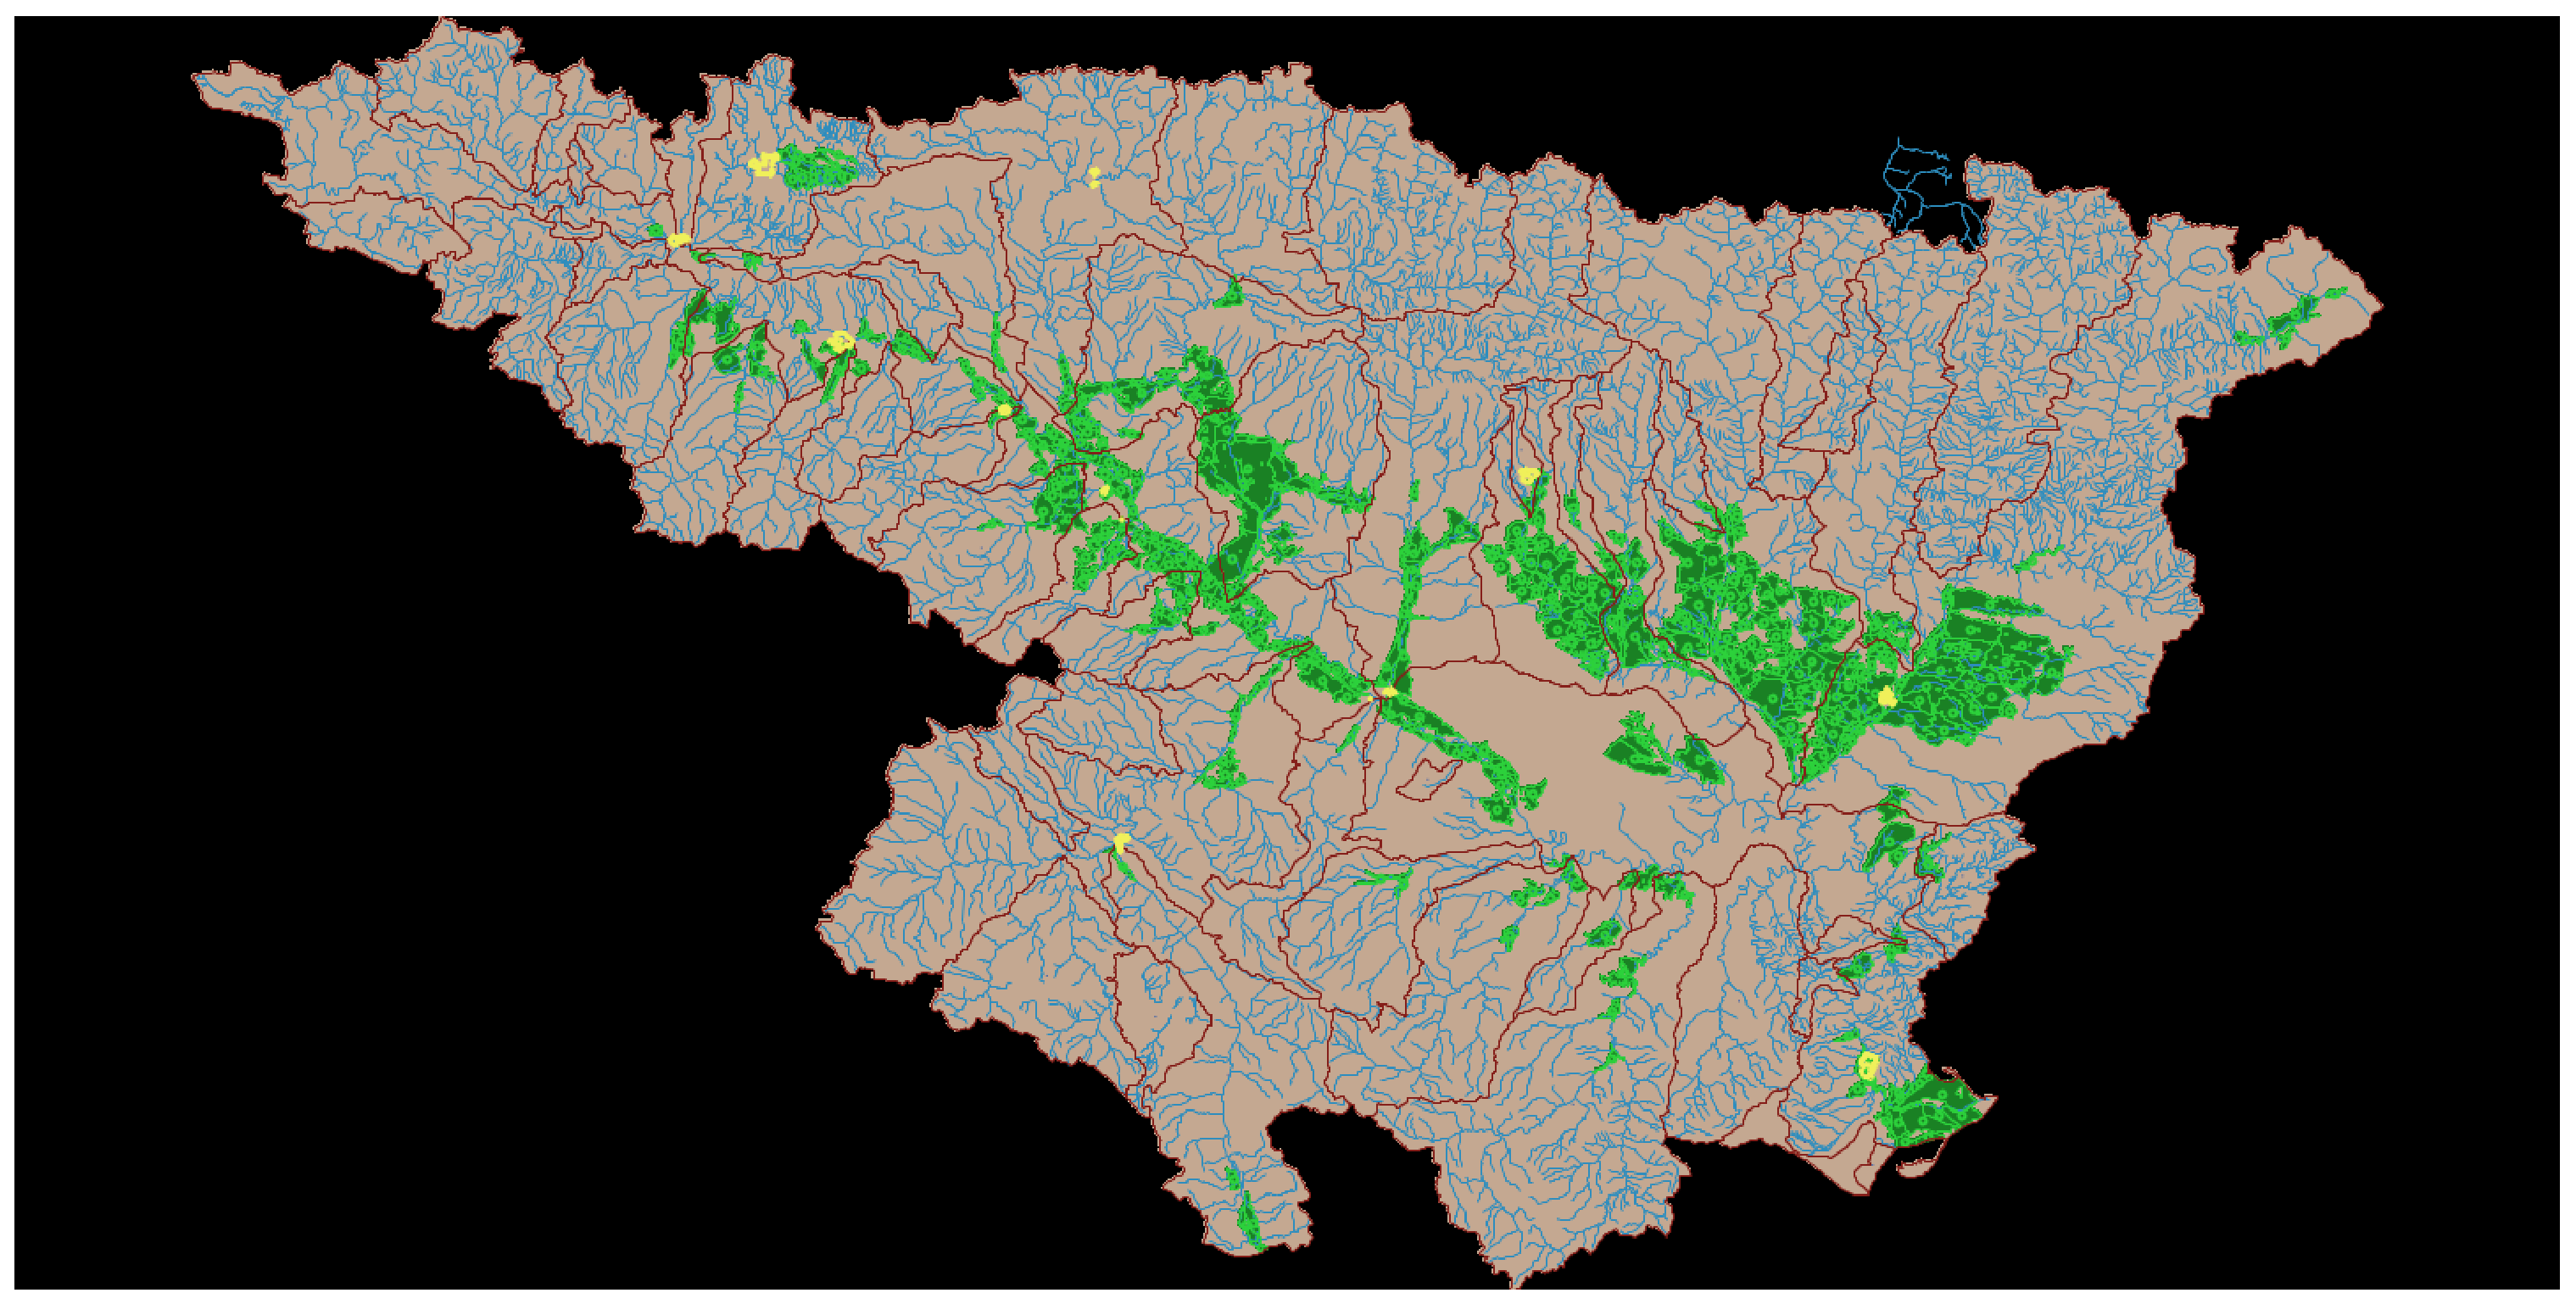
\includegraphics[width=\textwidth]{./world}
\caption{Darstellung der Modellumgebung}
\label{fig:world}
\end{figure}

Flussverl"aufe, Einzugsgebiete, bew"asserte Fl"achen und st"adtische Gebiete werden von der spanischen Hydrographischen Föderation Ebro \footnote{http://oph.chebro.es/ContenidoCartografico.htm} bezogen. Der j"ahrliche Verlauf der Wasserf"uhrung des Ebro wird von der UNH / GRDC (Global Runoff Data Centre) Gew"asserdatenbank \footnote{http://www.grdc.sr.unh.edu/html/Polygons/P6226800.html} bezogen. Die GIS-Daten, Bev"olkerungsdaten sowie hydrogeographischen Informationen wurden f"ur das Jahr 2006 gew"ahlt, um eine m"oglichst synchrone Datenbasis zu haben. Temperaturwerte (Anhang \ref{fig:ebro-temperatur}) werden von der World Meteorological Organization bezogen\footnote{http://worldweather.wmo.int/083/c01240.htm}.\\
Die Bev"olkerungsdaten stammen aus unterschiedlichen Quellen. Die Ver\-m"o\-gens\-ver\-teilung (\ref{fig:wealth-distribution}) wurde stochastisch nach den Angaben von \cite{Arbues2010} erstellt. Die Zusammensetzung der Haushalte (Anhang \ref{fig:hh-size-distribution}) wurde aus \cite{Barberan2007} entnommen.


\subsection{Simulation der Umwelt}\label{sec:Umweltfunktion}

In diesem Prozess werden die Umweltparameter festgelegt, die in diesem Zeitschritt gelten. Eine Funktion legt die Temperatur $T_{t}$ fest, die sich um den Monatsdurchschnitt verteilt verh"alt. Zur Festlegung der Wasserf"uhrungsmenge der Fl"usse (haupts"achlich des Ebro) $E_{t}$ l"auft ebenfalls eine Zufallsfunktion (\ref{eq:environment}) ab, die sich an den historischen Durchschnittsmengen $E_{n,t}$ der aktuellen Periode $t$ orientiert, und mit einem normalverteiltem Zufallsfaktor zwischen $0.75 < \xi < 1.25$ variiert. \\

\begin{dmath}
T_{t} = T_{n,t} * \xi
\label{eq:temperature}
\end{dmath}


\begin{dmath}
E_{t} = E_{n,t} * \xi
\label{eq:environment}
\end{dmath}

Die Wasserf"uhrung des Ebro ist ein zuf"alliger Wert, der mit einer Standardabweichung um Mittelwert des jeweiligen Monats schwankt (\ref{fig:ebro-water}). Mit einer Wahrscheinlichkeit, die als Modellparameter einstellbar ist (zwischen 0 und 25 Prozent), herrscht in einem bestimmten Jahr eine D"urre vor. In diesem Modell wird in solchen F"allen die normale Wasserf"uhrung auf einen Wert zwischen 40 und 60 Prozent der urspr"unglichen Menge reduziert.\\
Es kann ebenfalls eine Mindestf"uhrungsmenge eingestellt werden, ab deren Unterschreitung schwerwiegende "okologische Folgen drohen \citep{Alcacer2005}. Diese kann variiert werden, um Entscheidungstr"agern einen Trade-Off zu erm"oglichen zwischen der Gew"ahrleistung von Wasserangebot und Umweltqualit"at. Die Auswirkungen auf die Umwelt von sich "andernden Mindestf"uhrungsmengen werden in diesem Modell nicht betrachtet.

Alle Umweltparameter lassen sich gem"aß bestimmter Klimaprognosen mit einem beliebigen langfristigen Trend versehen. Sowohl Zu- oder Abnahme von Durchschnittstemperaturen, Zu- oder Abnahme der durchschnittlichen Wasserf"uhrungsmenge, oder die Zunahme der Variabilität (st"arkere Schwankungen der Temperatur, oder Zunahme von D"urreperioden) lassen sich in das Modell integrieren. Im einfachsten Szenario werden diese Trends nicht einbezogen. \\


\subsection{Angebotsfunktion}\label{sec:Angebotsfunktion}

Die Angebotsfunktion berechnet zum einen die physikalisch vorhandene Menge an Wasser, die zum einen als Stromgr"oße der aktuellen Wasserf"uhrung des Ebro vorliegt, zum anderen als Bestandsgr"oße an gespeichertem Wasser in Reservoirs.


\begin{tabular}{|c|c|c|}
\hline \textbf{Angebot} & & \\ 
\hline \textbf{Variablen} & \textbf{Typ} & Beispielwerte\\ 
\hline frei allokierbare Wassermenge & numerisch & 0 - 500 $Hm^3$ / Zeitschritt \\ 
\hline Speicher & numerisch & 0 - 6.837 $Hm^3$ \\ 
\hline \textbf{Funktionen} & & \\ 
\hline Angebotsfunktion & & Funktion \ref{eq:supply-function} \\
\hline Preisfunktion & & Funktion \ref{eq:household-price-function}\\
\hline 
\end{tabular} 


Die Existenz von Speichersystemen ist eine wichtige Funktion des Angebots. Vor allem in Gebieten mit saisonal stark schwankendem nat"urlichem Wasserangebot sind technische L"osungen notwendig um f"ur Ausgleich zu sorgen. Im Ebrogebiet wurden dazu Speicherkapazit"aten von 6.837 $Hm^3$ angelegt \citep{Penagos2007}. Im Modell ist es m"oglich, diese Kapazit"aten einmalig um einen Wert von 10 Prozent auszubauen. Dies soll wiederspiegeln, dass der Ausbau von Speicherkapazit"aten eine Option ist, die allerdings an ihre nat"urlichen und technologischen Grenzen stoßen kann und mit erheblichem Aufwand verbunden ist. Daher ist dieser Schritt nur einmalig um einen relativ geringen Wert m"oglich und wird erst im zehnten Modelljahr ausgef"uhrt, sollte diese Option im Modell aktiviert sein.


\begin{dmath}
Speicher_{(t)} = Speicher_{(t-1)} + (gef"uhrte\:Wassermenge_{(t)} - Mindestf"uhrungsmenge_{(t)}) - (urbane\:Nachfrage_{(t)} + landwirtschaftliche\:Nachfrage_{(t)})
\label{eq:supply-function}
\end{dmath}

Die Preisfunktion des Angebots f"ur Haushalte ist linear und ist dem Kostenmodell der Stadtverwaltung von Saragossa nachempfunden\footnote{http://www.zaragoza.es/contenidos/normativa/ordenanzas-fiscales/2013/OF_24-25-2013.pdf}. Haushalte zahlen f"ur die gesamte verbrauchte Wassermenge einen bestimmten Kubikmeterpreis, der dem Grenzpreis des letzten Kubikmeters entspricht.\\
\begin{dmath}
P_{w} = 
	\begin{array}{l l}
	0,210 & \quad \text{bis zu einem Verbrauch von 0,2 Kubikmeter / Tag}\\
	0,503 & \quad \text{bis zu einem Verbrauch von 0,616 Kubikmeter / Tag}\\
	1,258 & \quad \text{"uber einem Verbrauch von 0,616 Kubikmeter / Tag}
	\end{array}
\label{eq:household-price-function}
\end{dmath}

Im Rahmen dieser Arbeit ließ sich keine Preisfunktion aufstellen, die auf beide Akteure anwendbar ist. Dies liegt vor allem daran, dass das Wasser im Ebro f"ur Haushalte und Bew"asserungslandwirtschaften nicht das gleiche ist. W"ahrend sowohl Landwirtschaft als auch Haushalte vor allem vom Oberfl"achenwasser abh"angig sind, wird das Wasser f"ur st"adtische VerbraucherInnen in aufwendigen und kostspieligen Prozessen qualitativ aufbereitet. Das Wasser des Ebro ist im Grundzustand nicht als Trinkwasser geeignet \citep{Penagos2007}. Wasser zu Bew"asserung wird entweder aus Speichern, Kan"alen oder Fl"ussen direkt entnommen.

\subsection{Nachfragefunktion der Haushalte}\label{sec:Nachfrage-hh}

Die Nachfragefunktion entspricht der von \cite{Arbues2010} entworfenen Nachfragefunktion. Sie wurde deshalb gew"ahlt, weil sie zum Einen den Eingangs erw"ahnten Anforderung von \cite{Olmstead2010} entspricht (sie enth"alt Grenzpreise, Einkommen, Variablen f"ur Haushaltspr"aferenzen, Wettereinfl"usse), und zum Anderen weil sie speziell f"ur das Ebro-Becken entworfen wurde.\\

\begin{dmath}
ln q_{it} = \beta_{0} + \delta_{1}de_{it-2} + \delta_{2}(D1_{it} \times de_{it-2}) + \delta_{3}(D2_{it} \times de_{it-2}) + \delta_{4}(D3_{it} \times de_{it-2}) + \delta_{5}(D4_{it} \times de_{it-2}) + \delta_{6}HD_{it} + \delta_{7}ln q_{it-4}  + \beta_{1}W_{it} + \beta_{2}CHW_{it} + \beta_{3}AG20_{it} + \beta_{4}AG60_{it} + u_{it}
\label{eq:household-demand}
\end{dmath}

$lnq_{it}$ ist der Logarithmus des Haushaltskonsums. $\beta_{0-4}$ und $\delta_{1-7}$ sind Koeffizienten, die von \cite{Arbues2010} in ihrer Studie berechnet wurden (\ref{tab:elasticities}). Subskript \textit{it-x} steht für die jeweilige Zeitperiode. \textit{it} ist die aktuelle Periode, \textit{it-2} ist die zwei Perioden verz"ogert, um die Informationsverz"ogerung des Rechnungserhalts zu ber"ucksichtigen. Dies ist dadurch bedingt, dass Haushalte in dieser Region Informationen "uber ihren tats"achlichen Verbrauch und angefallene Kosten von ihren Versorgungsunternehmen um zwei Quartale verz"ogert erhalten. \textit{it-4} bezeichnet eine Verz"ogerung um vier Perioden, und gibt den Einfluss der gleichen Periode des Vorjahres wieder.\\
In dieser Funktion steht $\beta_{0}$ f"ur eine Konstante, $DN_{1-5}$ entsprechen Dummy-Variablen die Haushaltsgr"oßen repr"asentieren. HD ist eine Dummy-Variable f"ur Tage mit einer Maximaltemperatur von mehr als 18\celsius. CHW ist ebenfalls eine Dummy-Variable, die den Zugang zu einer gemeinsam genutzten Warmwasserquelle kennzeichnet. AG20 und AG60 sind Dummy-Variablen, die das Vorhandensein von Mitgliedern unter 20, respektive "uber 60 Jahren in einem Haushalt kennzeichnen. $de_{it-2}$ ist eine um zwei Perioden verz"ogerte Variable f"ur die Kosten der letzten Wasserrechnung, $\delta_{it-4}$ entspricht den Kosten aus dem gleichen Zeitraum des Vorjahres. Haushalte können aufgrund der linearen Preisfunktion (\ref{eq:household-price-function}) ihren Kubikmeterpreis nur nachtr"aglich ablesen, wenn ihr Verbrauch abgelesen wurde. Die Variable W entspricht dem Wohlstand des Haushalts, der approximiert "uber den Wert des bewohnten Eigentums einberechnet wird. Formel (\ref{eq:household-demand}) ist bereits auf die verschiedenen Haushaltsgr"oßen ausmultipliziert. Preiselastizit"at wird in dieser Funktion nicht explizit angef"uhrt, sondern fließt "uber die Variablen $de_{it-2}$ und $de_{it-4}$ ein.\\
\cite{Arbues2010} geben als Ergebnis ihrer Studie folgende Werte an:


\begin{table}[h]
\begin{tabular}{|c|r|l|l|}
\hline \textbf{Koeffizient} & \textbf{Wert} & \textbf{Variable} & \textbf{Erl"auterung}\\
\hline $\beta_0$ & -0.7026 &  & Konstante \\
\hline $\delta_1$ & -0.2645 & $de_{it-2}$ & Kosten (2 Perioden verschoben)\\
\hline $\delta_2$ & -1.0525 & D1 & Haushaltsgr"oße\\
\hline $\delta_3$ & -0.9509 & D2 & Haushaltsgr"oße\\
\hline $\delta_4$ & -0.1983 & D3 & Haushaltsgr"oße\\
\hline $\delta_5$ & -0.0078 & D4 & Haushaltsgr"oße\\
\hline $\delta_6$ & -0.0409 & HD & heiße Tage \\
\hline $\delta_7$ & 0.3228 & $de_{it-4}$ & Vorjahreskosten\\
\hline $\beta_1$ & 0.2941 $\times$ $10^{-5}$ & W & Verm"ogen\\
\hline $\beta_2$ & -0.1087 & CHW & Heißwasserversorgung\\
\hline $\beta_3$ & 0.0684 & AG20 & Altersvariable\\
\hline $\beta_4$ & -0.0692 & AG60 & Altersvariable\\
\hline
\end{tabular}
\caption{Elastizit"aten}
\label{tab:elasticities}
\end{table}


Die in Tabelle \ref{tab:elasticities} enthaltenen Elastizit"aten geben an, welchen Einfluss verschiedene Eigenschaften eines Haushalts auf das Verbrauchsverhalten haben. Die Variable $DN_{5}$ f"ur kommt deshalb nicht vor, da sie als Kontrollvariable f"ur $DN_{1-4}$ verwendet wurde. Haushalte mit f"unf oder mehr BewohnerInnen gehen also nur "uber den Koeffizienten  $\delta_1$ in die Formel ein. \\
Bei der Umsetzung im Modell ist darauf zu achten, dass Arbues et al. den Logarithmus des Verbrauchs formulieren. Um tats"achliche Werte zu erhalten, muss das Ergebnis in den Exponenten zu $e$ gehoben werden.\\


\subsection{Nachfragefunktion der Landwirtschaft}\label{sec: Nachfrage-LL}
Die Nachfragefunktion f"ur landwirtschaftlichen Wasserverbrauch (\ref{eq:irrigation-demand-function}) ist anderen Gesetzm"aßigkeiten unterworfen, da Wasser hier als Produktionsinput betrachtet werden kann. In erster Linie wird der Wasserverbrauch pro Bew"asserungslandwirtschaft als konstant pro Hektar Anbaufl"ache angenommen, und entspricht den Durchschnittswerten, die \cite{Salvador2011} festgestellt haben. In ihrer Studie sammelten sie Daten "uber eine repr"asentative Teilmenge von 10.475 ha. Da diese Werte nur "uber die gesamte Anbauperiode aggregiert vorhanden sind, ist es notwendig diese zu interpolieren, um so einen w"ochentlichen Bedarf festzulegen (Tabelle \ref{tab:waterproductivity}). Um nicht unn"otige Komplexit"at zu Beginn zu erzeugen, werden nur die vier im Ebro-Becken haupts"achlich angebauten Nutzpflanzen in das Modell aufgenommen: Mais mit 6.342 ha Anbaufl"ache, Alfalfa mit 1.994 ha Anbaufl"ache, Olivenb"aume mit 445 ha Anbaufl"ache und Tomaten mit 340 ha Anbaufl"ache. In Summe werden sie auf 87 Prozent (9.123 ha) der betrachteten 10.475 ha Anbaufl"ache im Ebro-Becken angebaut. F"ur die Modellberechnung werden diese Verteilungen auf die Gesamtfl"ache "ubertragen.\\

\begin{table}[h]
\begin{tabular}{|l|r|r|r|}
\hline Nutzpflanze & Fl"ache & Wasserbedarf IWA & Wasserproduktivit"at (Netto) \\ 
\hline & (ha) & ($m^{3}ha^{-1}$ ) & Euro $m^{-3}$ \\
\hline Mais & 6.342 & 7.199 & 0,13 \\ 
\hline Alfalfa & 1.994 & 8.823 & 0,83 \\ 
\hline Oliven & 445 & 2.878 & 0,42 \\ 
\hline Tomaten & 340 & 5.394 & 1,20 \\ 
\hline 
\end{tabular} 
\caption{Wasserbedarf und -produktivit"at}
\label{tab:waterproductivity}
\end{table}

Salvador et al. kalkulieren die "okonomische Nettoproduktivit"at von Wasser $WP_{En}$ als Verh"altnis von marginalem Nettoertrag (Einnahmen abz"uglich Kosten) einer Feldfrucht $M_{g}$ zu saisonalem Bew"asserungsvolumen IWA (Irrigation Water Applied, Formel (\ref{eq:waterproductivity})). Die Bew"asserungsperiode wird von Mai bis September angenommen. Im Modell wird daher der saisonale Wasserbedarf IWA durch die Anzahl der Wochen (25) geteilt und durch eine Dummy-Variable $I$ dargestellt, die den Wert 0 annimmt, wenn nicht bew"assert wird, und 1, wenn bew"assert wird.\\

Der Preis von Wasser, das in der Landwirtschaft verwendet wird, l"asst sich nach \cite{George2011a} anhand des Grenzproduktes festlegen. Der Wert des Grenzproduktes von Wasser (WP) ist als sein Wert als Produktionsfaktor zu sehen, und ist daher vor allem vom produzierten Gut abh"angig. F"ur das Wassereinzugsgebiet des Ebro haben (\cite{Salvador2011}) die Grenzproduktivit"at von Wasser bez"uglich verschiedener Endprodukte sowie Bew"asserungstechniken gesch"atzt (s. Tabelle \ref{tab:waterproductivity}).\\

\begin{dmath}
WP_{En} = \frac{M_{n}}{IWA}
\label{eq:waterproductivity}
\end{dmath}

\begin{dmath}
q_{ir} = \frac{IWA}{25 * Fl"ache * I}
\label{eq:irrigation-demand-function}
\end{dmath}

\subsection{Knappheit}
\label{Knappheitsfunktion}

Knappheit tritt in diesem Modell dann auf, wenn aufgrund dauerhaft nie\-drig\-er Pegelst"ande die Nachfrage der Haushalte und Landwirtschaften die Wasserspeicher vollkommen entleert haben. Dies ist ein Extremzustand und dient in diesem Modell auch der Vereinfachung. Die zur Verf"ugung stehende Menge Wasser beschr"ankt sich nun auf das im Ebro vorhande. Unter Ber"ucksichtung bestimmter Pegelst"ande, die nicht unterschritten werden sollten, bleibt so nur eine Restmenge Wasser "ubrig, die auf die KonsumentInnen und Landwirtschaften verteilt werden muss.\\
Knappheit wird in diesem Fall als Verh"altnis von nachgefragter zu phy\-sisch vorhandener Menge ausgedr"uckt. In diesem Modell wird als einfachster regulatorischer Eingriff unter Knappheit eine Mengenreduktion umgesetzt. Dabei wird die Menge an Wasser, die "uber das verf"ugbare hinausgeht, anteilsm"aßig auf alle Haushalte und Landwirtschaften verteilt. Dabei wird eine relative Gleichbelastung erzeugt, keine absolute. Das bedeutet, dass ein Haushalt seinen Konsum nicht um einen absoluten Betrag in Kubikmetern einschr"anken muss, der f"ur alle gleich ist, sondern um einen Prozentsatz der f"ur alle Haushalte gleich ist.\\

\begin{dmath}
s_{(t)} = \frac{urbane\:Nachfrage_{(t)} + landwirtschaftliche\:Nachfrage_{(t)}}{gef"uhrte\:Wassermenge_{(t)}}
\label{eq:scarcity-function}
\end{dmath}


\subsection{Nutzenfunktionen}
\label{Nutzenfunktion}

Zur Messung der Auswirkungen einer Wasserknappheit werden die Nutzenfunktionen herangezogen, die im folgenden beschrieben werden. Sie berechnen nun anhand der einem Haushalt oder einer Landwirtschaft zur Verf"ugung stehenden Wassermenge den Nutzen, der aus dem Verbrauch dieses Wassers generiert werden kann. Dabei werden parallel der Nutzen im Normalfall und der Nutzen unter Knappheit berechnet, d.h. f"ur den Fall dass der Wasserkonsum rationiert werden muss. Im n"achsten Schritt wird der Knappheitsnutzen vom normalen Nutzen abgezogen. Das Ergebnis ist der Nutzenverlust. Umweltpolitische Steuerungsmaßnahmen k"onnen dahingehend eval\-uiert werden, ob sie diesen Nutzenverlust minimieren k"onnen.\\

Die Nutzenfunktion der Haushalte ist relativ einfach gehalten und berechnet f"ur jeden Haushalt den Nutzen anhand des Konsums, der Haushaltsgr"oße und des gezahlten Preises. Der Preis fließt hier in die Funktion ein, da er als Indikator f"ur die Wertsch"atzung von Wasser gesehen werden kann.

\begin{dmath}
U_{h} = q_{it} * DN * TF^{2} * Preis
\label{eq:household-utility-function}
\end{dmath}

Die Nutzenfunktion ist ebenfalls einfach gestaltet und berechnet den Nutzen einer Landwirtschaft $U_{ir}$ aus der Grenzproduktivit"at $WP_{En}$, der zugef"uhrten Wassermenge IWA und der Fl"ache. I ist die Dummy-Variable die die Bew"asserungsperiode anzeigt.

\begin{dmath}
U_{ir} = \frac{IWA * WP_{En} * I}{25 * Fl"ache} = \frac{M_{n} * I}{25 * Fl"ache}
\label{eq:irrigation-utility-function}
\end{dmath}

\subsection{Lernfunktionen}

Das Auftreten von Knappheiten kann bei den AkteurInnen zu Verhaltens\-"and\-erungen f"uhren, weil sie nach Wegen suchen, ihren Nutzen in der neuen Situation zu maximieren. Einer der einfachsten Wege, wie Lern- und Entscheidungsverhalten in einem agentenbasierten Modell dargestellt werde kann, sind Heuristiken \citep{Rounsevell2012}. Sie folgen einem ,,falls ... dann ... sonst ...''-Schema. Der Vorteil hierbei ist, dass das Entscheidungsverhalten sehr transparent ist, und direkt aus konzeptionellen Entscheidungsb"aumen "ubertragen werden kann. In der Lernfunktion (\ref{eq:household-learning-function}) vergleicht sich ein Haushalt mit der Menge aller anderer Haushalte $M_{h}$, die h"oheren Nutzen bei geringen Kosten aufweisen. Danach vergleicht er innerhalb dieser Teilmenge die zwei Variablen, auf die er in diesem Modell Einfluss hat: Haushaltsgr"oße (DN) und technologische Effizienz (TF). Sollte der Mittelwert einer Variable innerhalb dieser Gruppe eine deutliche Tendenz aufweisen, entscheidet sich der Haushalt diese Variable zu "ubernehmen ($LD_{h}$ und $LT_{h}$). Dieses einfache adaptive Verhalten soll zum einen eine soziale Komponente - n"amlich den Einfluss der angestrebten Haushaltsgr"oße - und eine technische Komponente - die Verbesserung der Effizienz - enthalten. Dieses Modell ber"ucksichtigt allerdings weder die Informations- noch Transformationskosten, die f"ur diese Prozesse notwendig sind. Ein weiterer Aspekt der von Rounsevell et al. hervorgehoben wird, ist \textit{bounded rationality}. Das eingeschr"ankt vorhandene Wissen um die optimale L"osung wird in diesem Modell so wie von \cite{Rounsevell2012} beschrieben modelliert, in dem Haushalte nur eine Teilmenge der gesamten Alternativen betrachten.

\begin{dmath}
\begin{array}[h]{l}
M_{h} = alle\:Haushalte\:mit\:(Nutzen\:>\:eigener\:Nutzen)\\
\;\;\;\;\;\;\;\;\;\;\;UND\:(Kosten\:<\:eigene\:Kosten)\\
LD_{h} = setze\:Haushaltsgr"oße\:auf\:(Durchschnittswert\:von\:M_{h})\\
LT_{h} = setze\:Technologiefaktor\:auf\:(Durchschnittswert\:von\:M_{h})
\end{array}
\label{eq:household-learning-function}
\end{dmath}


Die Entscheidungsfunktion (\ref{eq:irrigation-learning-function}) der Landwirtschaften dient dazu, den zuk"unftigen Nutzen zu maximieren. Dazu erhalten Landwirtschaften ein ,,Ged"achtnis'' $dm$, das f"unf Jahre zur"uck reicht und das Auftreten von D"urre\-perioden speichert. Im Modell ist es einfach die Anzahl der D"urren innerhalb der letzten 5 Jahre. Unter der Annahme, dass Klima sich langfristig ver"andert, soll dies soll dazu dienen, die aktuellen Umweltzust"ande zu internalisieren. Landwirtschaften stellen dann f"ur jede Nutzpflanze die gleiche Berechnung an: Sie kalkulieren den m"oglichen Nutzen $S_{1-n}$ anhand der Produktivit"at pro Kubikmeter Wasser $WP_{En, 1-n}$, im Verh"altnis zur ben"otigten Menge $IWA_{1-n}$ und w"ahlen dann die erfolgversprechendste Pflanze. Der erwartete Nutzen wird mit dem Wert der in die Zukunft zu erwartenden D"urreh"aufigkeit $(1\:-\: dm * 0.2)^{5}$ multipliziert. Dadurch soll ein Verhalten simuliert werden, dass den Nutzen hinsichtlich der Versorgungsunsicherheit im Wasserverbrauch maximiert, um Ernteausf"alle zu vermeiden.\\


\begin{dmath}
S_{1-n} = \frac{WP_{En, 1-n} * (1\:-\: dm * 0.2)^{5}}{IWA_{1-n}}
\label{eq:irrigation-learning-function}
\end{dmath}

Dieses Verhalten wird auch von \cite{Varela-Ortega1998} beobachtet, welche schlussfolgern dass Bew"asserungslandwirtschaften auf ver"andertes Wasserangebot mit zwei Strategien reagieren: Bei Preissteigerungen wechseln sie auf weniger stark zu bew"assernde Nutzpflanzen. Es gibt auch einen Preis, bzw. Wasserverf"ugbarkeitsschwelle, ab welcher Trocken\-land\-wirt\-schaft kompetitiv ist. Ab diesem Zeitpunkt wird die Bew"asserung zugunsten einer Trockenlandwirtschaft aufgegeben.\\
Ebenso wie bei den Haushalten k"onnen innerhalb dieser Arbeit Informations- und Transformationskosten (z.B. durch Fruchtwechsel) nicht ber"ucksichtigt werden. Fruchtwechsel sind im Modell jedes Jahr m"oglich und es steht eine repr"asentative Auswahl an Nutzpflanzen zur Verf"ugung (Tabelle \ref{tab:waterproductivity}). Der Schritt eines Wechsels zu Trocken\-land\-wirt\-schaft wird in diesem Modell nicht simuliert, da hierf"ur weitere Daten hinsichtlich der Kompetitivit"at von Trockenlandwirtschaft notwendig w"aren.

\newpage

\section{Modelloutput und Interpretation}
\label{sec:Modelloutput}
Das Modell wird mit empirischen Daten initialisiert, die den aktuellen realen Zustand abbilden. Jede Kombination von Parametern kann mehrfach wiederholt werden. Insgesamt wurden zur Evaluierung des Modells 800 Durchl"aufe unter Variierung verschiedener Startparameter durchgef"uhrt. Die maximale Dauer eines Laufs betragt 1040 Zeitschritte, also 20 Jahre.

\begin{table}[h]
\begin{tabular}{|l|r|}
\hline \textbf{Parameter} & \textbf{Wertebereich} \\
\hline D"urrewahrscheinlichkeit & 0, 5, 10, 15, 20, 25 Prozent  \\ 
\hline Lernverhalten Haushalte & Nein / Ja  \\ 
\hline Lernverhalten Landwirtschaften & Nein / Ja \\ 
\hline minimale Wasserf"uhrung & 150 / 300 m$^{3}$s$^{-1}$  \\ 
\hline Speichererweiterung & 0 / 10 Prozent \\ 
\hline 
\end{tabular} 
\caption{Startparameter}
\label{tab:input-parameters}
\end{table}
\newline
\newline
\begin{table}[h]
\begin{tabular}{|l|}
\hline \textbf{beobachtete Variablen je Zeitschritt} \\
\hline Aggregierter Nutzen der Haushalte \\ 
\hline Aggregierter Nutzen der Landwirtschaften  \\ 
\hline Aggregierter Nutzen-Verlust der Haushalte  \\ 
\hline Aggregierter Nutzen-Verlust der Landwirtschaften  \\ 
\hline Durchschnittsnutzen der Haushalte  \\ 
\hline Durchschnittsnutzen der Landwirtschaften  \\ 
\hline Durchschnitts-Nutzenverlust der Haushalte  \\ 
\hline Durchschnitts-Nutzenverlust der Landwirtschaften  \\ 
\hline Wassermenge des Ebro  \\ 
\hline Wassermenge in Reservoirs \\ 
\hline Durchschnittsgr"oße der Haushalte  \\ 
\hline Verteilung der Nutzpflanzen  \\ 
\hline 
\end{tabular} 
\caption{Kennzahlen}
\label{tab:output-variables}
\end{table}

Das Modell speichert zu jeden Zeitschritt die in Tabelle \ref{tab:output-variables} angef"uhrten Variablen ab. In einem Testlauf ergab das Modell zur statistischen Analyse 916.000 Datenpunkte zu 12 Variablen. Grafik \ref{fig:ebro-wasser-output} visualisiert die Wasserf"uhrung des Ebro "uber den Zeitverlauf. Der Wert allokierbares Wasser nimmt hier in D"urreperioden maximale Fehlmengen von mehr als 100 $Hm^{3}$ an. Dies sind Mengen, die entweder eingespart werden m"ussen, oder durch Absenkung der Mindestf"uhrungsmenge aus der nat"urlichen Reserve zus"atzlich entnommen werden.

\begin{figure}[h]
\centering
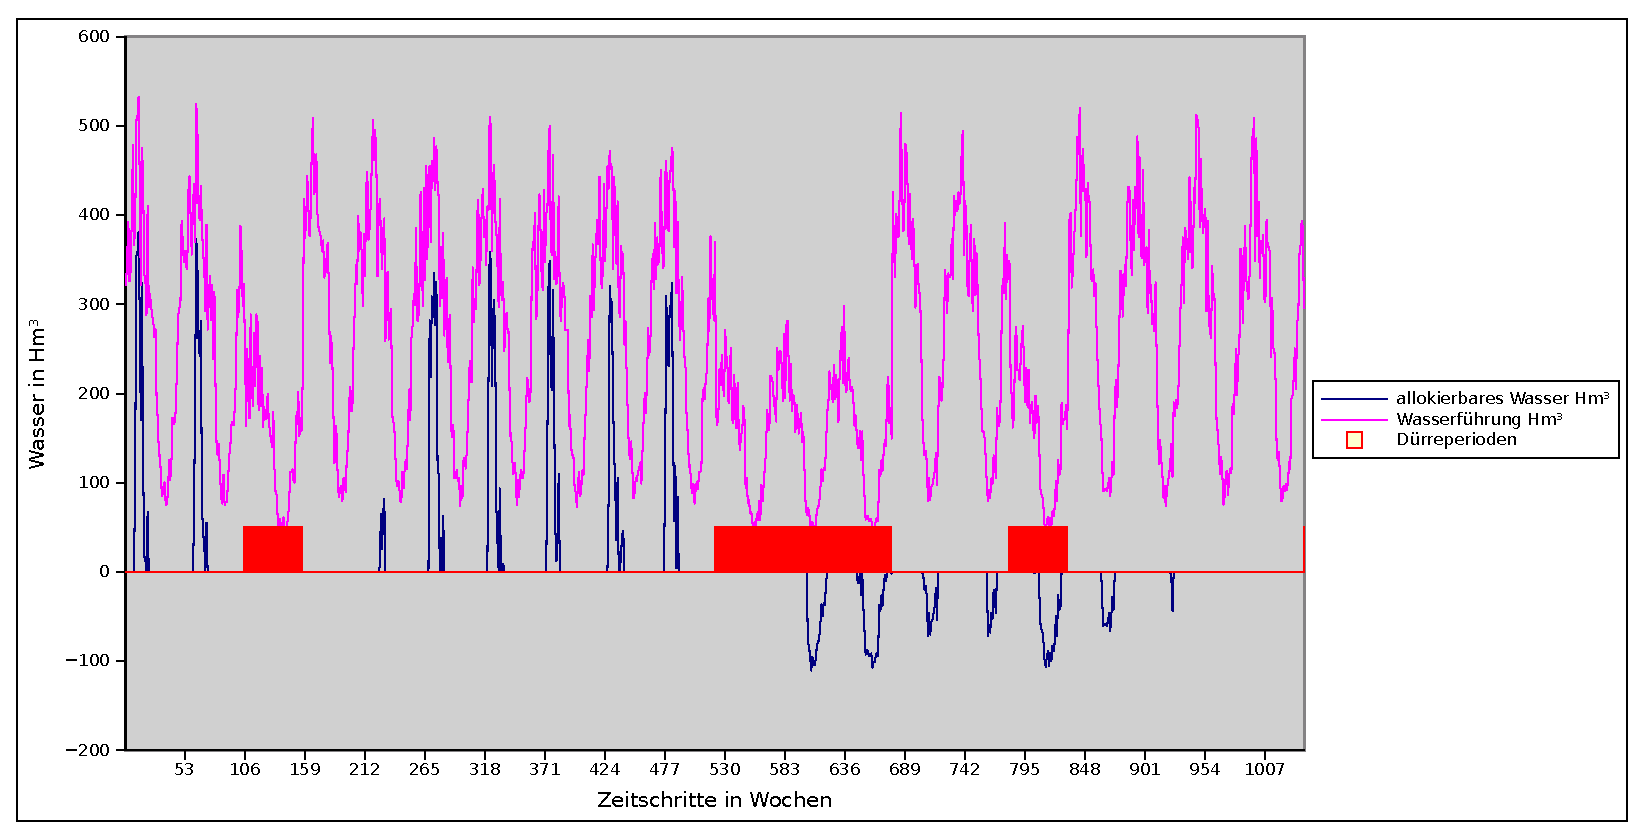
\includegraphics[width=\textwidth]{./ebro-wasser-output}
\caption{Wasserf"uhrung und allokierbares Wasser}
\label{fig:ebro-wasser-output}
\end{figure}



Grafik \ref{fig:demandpc} stellt einen exemplarischen Verlauf der Variable pro-Kopf-Verbrauch dar. In dieser Konfiguration waren alle Lernfunktionen aktiviert. Der pro-Kopf-Verbrauch sinkt hier von einem Anfangswert von 100 l / Tag auf 92 l / Tag.

\begin{figure}[h]
\centering
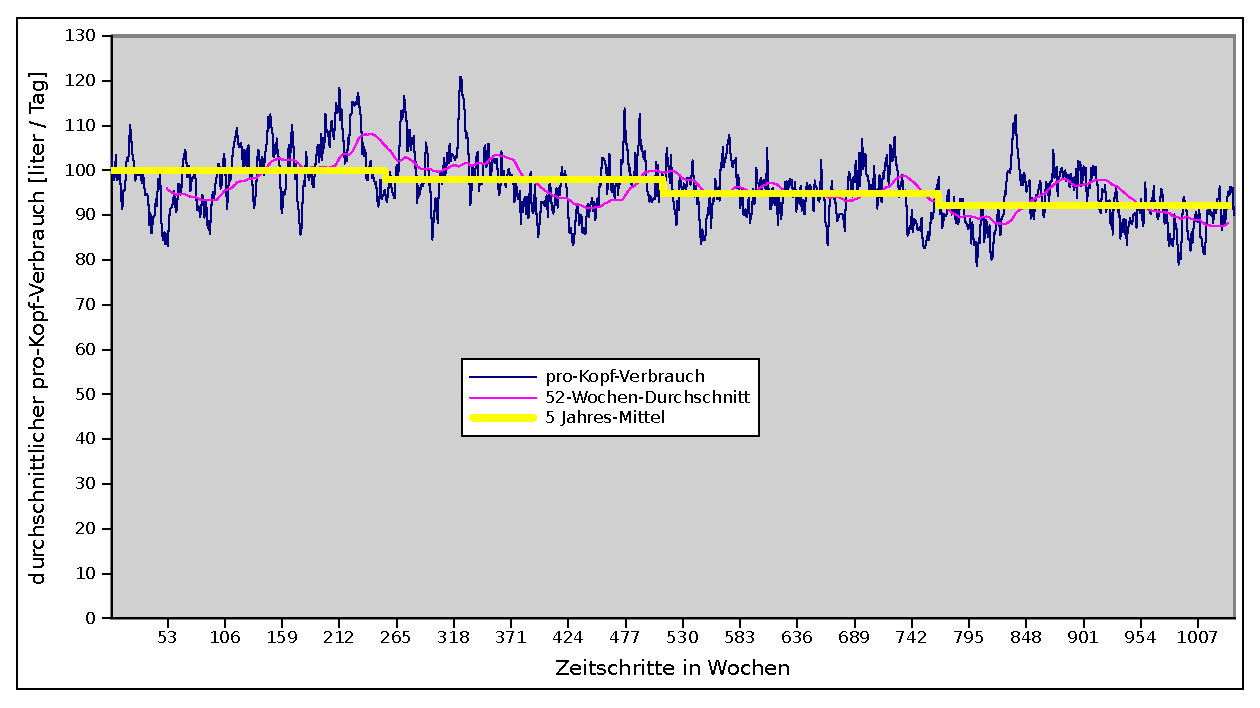
\includegraphics[width=\textwidth]{./demandpc}
\caption{pro-Kopf-Verbrauch}
\label{fig:demandpc}
\end{figure}


\cite{Arbues2010} kommen zu der Beobachtung, dass es drei verschiedene Verbrauchsmuster gibt - eines f"ur kleine Haushalte mit einem oder zwei Mitgliedern, eines f"ur mittlere Haushalte mit 3 Mitgliedern und eines f"ur große Haushalte mit vier oder mehr BewohnerInnen. Sie f"uhren dies im wesentlichen auf zwei Gr"unde zur"uck:
\begin{itemize}
\item Endogene Transaktionskosten stehen der Einf"uhrung von neuen Techniken oder Verhaltensweisen entgegen, und sind in gr"oßeren Haushalten h"oher. Die Komplexit"at der Organisation von Haushalten und die Umsetzung neuer Praktiken steigt mit der Gr"oße und wirkt sich auch auf Entscheidungsprozesse aus. Transaktionskosten (Fehlen von Informationen, Fehlanreize, heterogene BewohnerInnen, Monitoringkosten, Gewohnheiten) steigen und erschweren die Umsetzung von Wassersparmaßnahmen im Vergleich mit kleineren Haushalten.
\item Demgegen"uber wirken Skaleneffekte vorteilhaft: In kleineren Haushalten (1-2 BewohnerInnen) kommt es zu Ineffizienzen zum Beispiel bei der Nutzung von Geschirrsp"ul- und Waschmaschinen, die tendenziell unter der maximalen Kapazit"at laufen. Gr"oßere Haushalte k"onnen in der Nutzung eine h"ohere Effizienz erreichen und so trotz absolut h"oherem Verbrauch niedrigere pro-Kopf-Verbr"auche erreichen.
\end{itemize}
Diese Beobachtungen decken sich mit den Ergebnissen des Modells, die ein prinzipielles konvergieren auf zwei Haushaltsgr"oßen mit entweder einem oder 3 BewohnerInnen zeigen. Diese Ergebnisse sind nat"urlich nur als Tendenzen zu sehen, da in der Realit"at wesentlich mehr Einflussfaktoren vorherrschen. Innerhalb dieser Arbeit zeigt sich hinsichtlich des Umgangs mit Knappheiten zwei unterschiedliche Gruppen von WasserkonsumentInnen gibt.\\

Bei den Landwirtschaften gibt es ein interessantes Ph"anomen zu beobachten. Von den vier eingebauten Nutzpflanzen bleiben nach kurzer Zeit nur noch zwei relevant: Mais und Tomaten. Wie in Grafik \ref{fig:crop-types} dargestellt ist, steigt in Phasen regelm"aßiger Wasserversorgung der Tomatenanbau best"andig an. Da Tomaten einen niedrigeren Wasserbedarf haben, sinkt der durchschnittliche Wasserbedarf der Farmen. (Tabelle \ref{tab:waterproductivity}). Ab ca. Woche 520 herrscht f"ur drei Jahre eine D"urreperiode vor, und hat sofort Auswirkungen auf die strategischen Entscheidungen der LandwirtInnen. In den n"achsten 5 Jahren steigt der Maisanbau rapide an, w"ahrend der Tomatenanbau abnimmt. Dies ist auf den ersten Blick eine widerspr"uchliche Entwicklung, da Mais einen h"oheren Wasserbedarf hat als Tomaten. Betrachtet man allerdings die Grenzproduktivit"aten wird klar, dass dahinter eine strategische Entscheidung steht. Tomaten haben zwar einen h"oheren Ertrag, dieser ist allerdings auch mit h"oheren Investitionen verbunden - manuelle Pflege und Ernte verteuern den Tomatenanbau im Vergleich zum maschinell bearbeitbaren Mais. In Zeiten unsicherer Wasserversorgung erscheinen Tomaten daher als riskantere Investition, w"ahrend beim Mais m"ogliche Verluste geringer sind. Die problematische Entwicklung dabei ist, dass mit Mais der Durchschnittsverbrauch wieder ansteigt, und so die Krise noch versch"arft werden kann.

\begin{figure}[h]
\centering
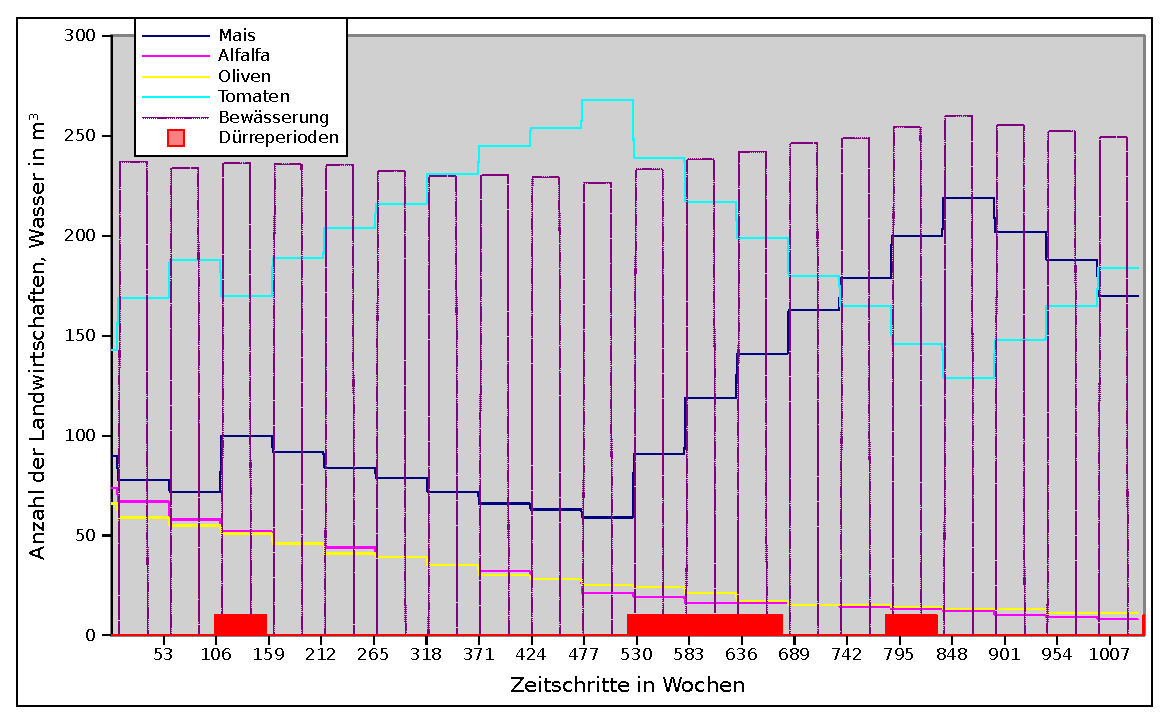
\includegraphics[width=\textwidth]{./crop-types}
\caption{Variation der Nutzpflanzen und Gesamtverbrauch}
\label{fig:crop-types}
\end{figure}

Wie in Grafik \ref{fig:utility-losses} zu sehen ist, f"uhren die strategischen Entscheidungen der landwirtschaften zu einer tendenziellen Reduktion von Nutzenverlusten. Dies kann als eine Steigerung der Resilienz interpretiert werden. Das sozio"okonomische System stellt sich auf ver"anderte Umweltbedingungen ein, passt seine Erwartungen und erreicht so einen anderen, stabilen Zustand. Inwiefern dies ein tats"achliches Ph"anomen ist, oder inwiefern durch umweltpolitische Maßnahmen diese Tendenzen verst"arkt werden k"onnen, geht "uber die Interpretationsm"oglichkeiten dieser Arbeit hinaus. 

\begin{figure}[h]
\centering
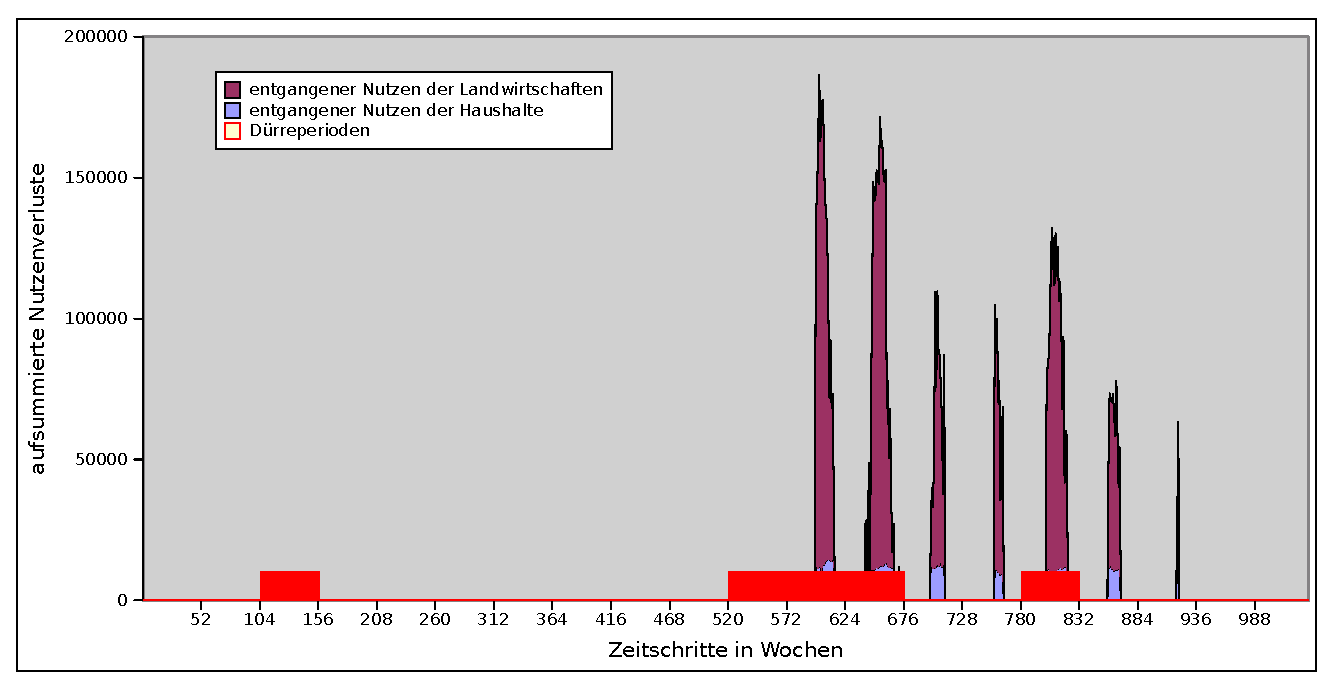
\includegraphics[width=\textwidth]{./utility-losses}
\caption{Nutzenverluste}
\label{fig:utility-losses}
\end{figure}

\newpage

\section{Schlussfolgerungen}
Erste Analysen lassen vermuten, dass nachfrageseitig die potenziellen Aus\-wir\-kungen auf den Wasserkonsum durch soziale Verhaltens"anderungen aus\-schlag\-gebend sind. Eine Analyse, ob technische Effizienzsteigerungen signifikant keine Aus\-wirkungen haben, oder ob auch hier das Ph"anomen der Affluenz zum Tragen kommt, steht noch aus. Dabei ist nat"urlich ganz klar zu betonen, dass beispielsweise die durchschnittliche Haushaltsgr"oße kein Wert ist, der durch Anschalten einer Funktion ver"andert werden kann. In diesem Modell rep"rasentiert sie eine nachfrageorientierte Policy, die auf einen bestimmten, empirisch beobachteten Einflussfaktor abzielt. In der Realit"at kann dies entweder durch Information und Bewusstseinsbildung der Bev"olkerung geschehen, aber auch durch finanzielle Anreize wie die Wohnbauf"orderung hinsichtlich gr"oßerer Wohneinheiten. Die Subventionierung wassereffizienter Haushaltstechnik ist ebenfalls ein Mittel das angewendet werden kann. In diesem Modell hat sich allerdings herausgestellt, dass technologische Faktoren weniger starken Einfluss auf Resilienz gegen"uber Knappheit hat.

Im Hinblick auf die systemische Natur umwelt"okonomischer Probleme ist auch Seitens der ModellentwicklerInnen ein starkes Zugehen auf Betroffene und Stakeholder n"otig und sinnvoll. Zum Einen sind sie von den Ergebnissen der Modelle betroffen, sollten diese im Rahmen von Policy-Einsch"atzungen entwickelt werden, zum Anderen k"onnen sie mit Experten- und Domainwissen zur Modellentwicklung beitragen. \cite{Leenhardt2012} und \cite{Scott2012} entwickelten dazu Frameworks.

"Uber die Modellentwicklung hinaus sollte in dieser Arbeit in einfachen Ans"atzen gezeigt werden, dass es m"oglich ist mit agentenbasierten Modellen die Anforderungen, die an eine Methodik zur Untersuchung "okonomischer Zusammenh"ange gestellt wird, prinzipiell zu erf"ullen. F"ur zuk"unftige Modellentwicklung ist ebenfalls erkennbar, dass die großen H"urden f"ur "ahnliche Projekte in der Beschaffung empirischer Daten liegen. Um agentenbasierte Modelle realit"atsnah zu implementieren, sind Mikrodaten notwendig. Hier ist nat"urlich Datenschutz ein kritischer Punkt, genauso wie die Eigentumsfrage an diesen, da solche Daten meist von privaten Unternehmen im Zuge ihrer wirtschaftlichen T"atigkeit erzeugt werden. Doch in den F"allen, in denen solche Daten durch "offentliche, von Steuergeldern finanzierte Institutionen erhoben werden, ist die Ver"offentlichung dieser Daten (anonymisiert) von einem wissenschaftlichen Standpunkt nach Prinzipien von Open Science und Open Data erw"unscht. Auch individuelle WissenschaftlerInnen k"onnen hierzu beitragen, wie es in den Panton-Prinzipien\footnote{http://pantonprinciples.org/} gefordert wird.\\

\section{Lizenz}

Dieses Werk ist lizenziert unter einer Creative Commons Namensnennung 4.0 International Lizenz.

\newpage


\bibliography{sources.bib}
\bibliographystyle{apalike}

\newpage

\appendix{Grafiken}

\begin{figure}[h]
\centering
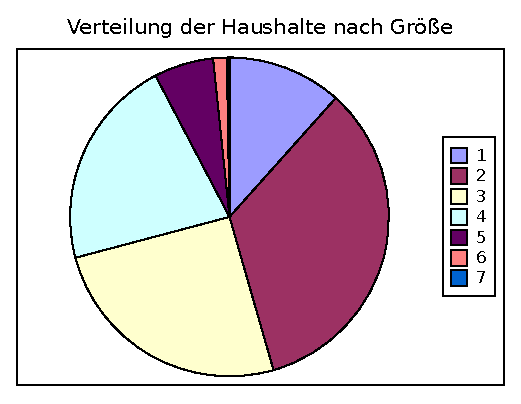
\includegraphics[width=\textwidth / 3 * 2]{./hh-size-distribution}
\caption{}
\label{fig:hh-size-distribution}
\end{figure}

\begin{tabular}[h]{|c|r|}
\hline Haushaltsgr"oße & prozentualer Anteil \\ 
\hline 1 & 11,61 \\ 
\hline 2 & 33,94 \\ 
\hline 3 & 25,33 \\ 
\hline 4 & 21,45 \\ 
\hline 5 & 6,03 \\ 
\hline 6 & 1,38 \\ 
\hline 7 & 0,27 \\ 
\hline 
\end{tabular} 

\begin{figure}[htbp]
\centering
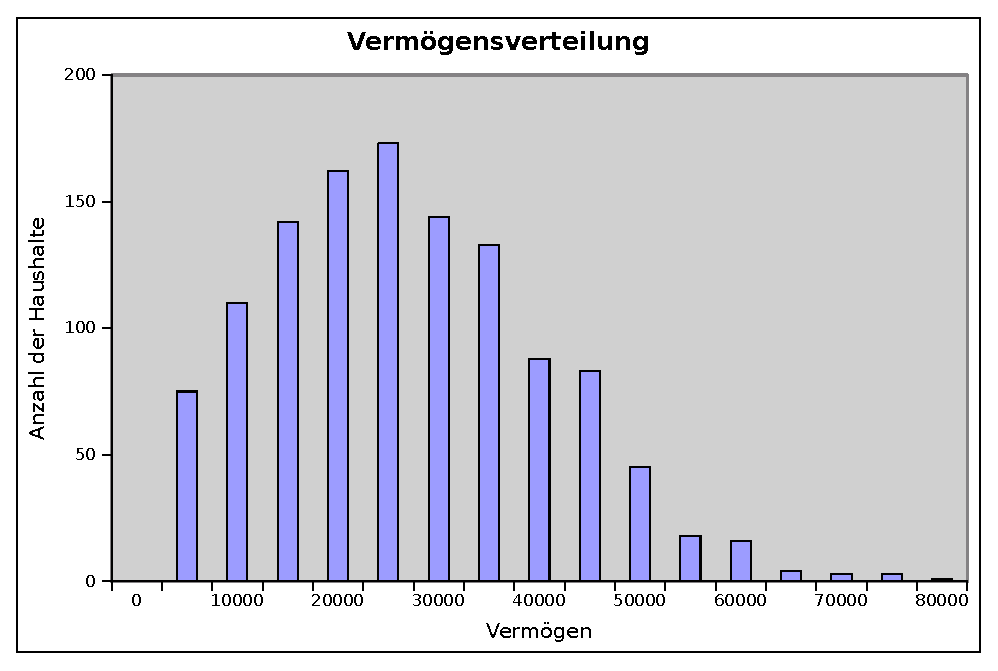
\includegraphics[width=\textwidth]{./wealth-distribution}
\caption{}
\label{fig:wealth-distribution}
\end{figure}

\begin{figure}[h]
\centering
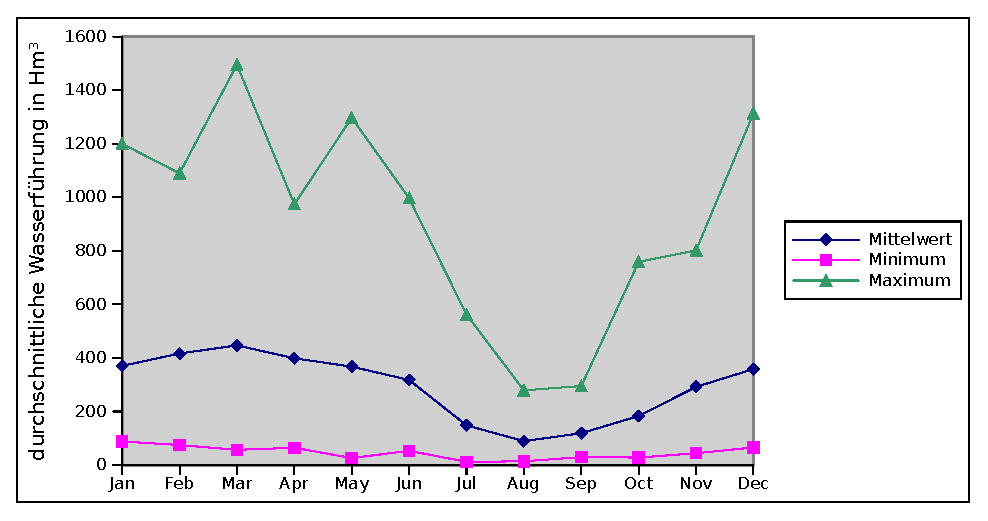
\includegraphics[width=\textwidth]{./ebro-wasser}
\caption{Wasserf"uhrung des Ebro im Jahresverlauf an der Messstation Tortosa, Angaben in Kubikhektometern (mio Kubikmeter)}, Quelle: UNH / GRDC Datenbank
\label{fig:ebro-water}
\end{figure}

\begin{figure}[h]
\centering
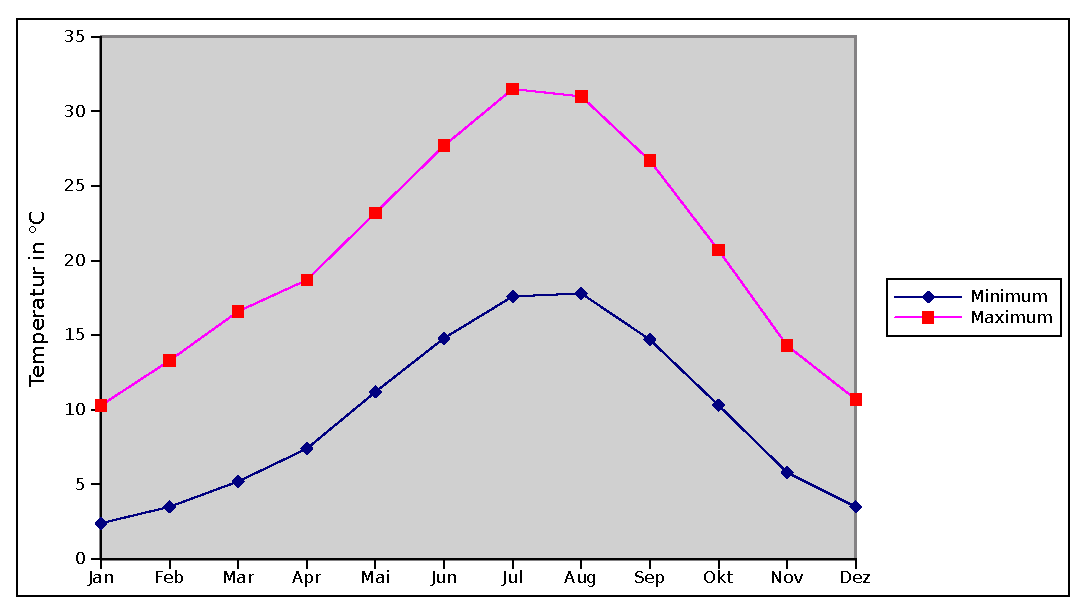
\includegraphics[width=\textwidth]{./ebro-temperatur}
\caption{Durchschnittliche Temperaturen im Ebro-Becken, Messstation Saragossa}
\label{fig:ebro-temperatur}
\end{figure}



\end{document}
